\pdfoutput=1
% ^ arXiv detects a pdflatex submission from this line; keep it within
%   the first five lines of the file.
\documentclass[10pt]{article}

\usepackage[biblatex]{flockpaper}

\usepackage{subcaption}
\usepackage{nicefrac}
\usepackage{algorithm2e}

\usepackage[backend=biber]{biblatex}
\addbibresource{refs.bib}
\renewcommand*{\bibfont}{\normalfont\small}

% allow long URLs in the bibliography to break across lines
\setcounter{biburlnumpenalty}{9000}
\setcounter{biburlucpenalty}{9000}
\setcounter{biburllcpenalty}{9000}

\usetikzlibrary{arrows.meta, bending, positioning}

\newcommand{\map}{\mathop{\bigoplus}\limits}
\newcommand{\txtop}[1]{\mathop{\mathtt{#1}}\limits}

\newcommand{\expr}{\txtop{expression}}

\newcommand{\fn}{\txtop{function}}
\newcommand{\linear}{\txtop{linear}}
\newcommand{\relu}{\txtop{ReLU}}
\newcommand{\topk}{\txtop{TopK}}
\newcommand{\sigmoid}{\txtop{sigmoid}}
\newcommand{\tanhl}{\txtop{tanh}}
\newcommand{\softmax}{\txtop{softmax}}
\newcommand{\argmin}{\txtop{argmin}}
\newcommand{\argmax}{\txtop{argmax}}
\newcommand{\einsum}{\txtop{einsum}}
\newcommand{\colsum}{\txtop{colsum}}

\newcommand{\encoder}{\txtop{encoder}}
\newcommand{\decoder}{\txtop{decoder}}
\newcommand{\classifier}{\txtop{classifier}}
\newcommand{\partitioner}{\txtop{dict}}

\newcommand{\bilinearblock}{\txtop{BilinearBlock}}
\newcommand{\dictblock}{\txtop{DictBlock}}
\newcommand{\dictenc}{\txtop{DictEnc}}
\newcommand{\ontologizer}{\txtop{Ontologizer}}

\SetKwProg{Fn}{Function}{}{end}
\SetKwProg{Dat}{Data}{}{end}

\SetKwInOut{Hyper}{Hyperparameters}

\SetKwFunction{softmax}{softmax}
\SetKwFunction{MSE}{MSE}
\SetKwFunction{L1}{L1}
\SetKwFunction{transpose}{transpose}
\SetKwFunction{matmul}{matmul}
\SetKwFunction{dist}{dist}
\SetKwFunction{eucl}{euclidean}
\SetKwFunction{cossim}{cossim}
\SetKwFunction{sindiff}{sindiff}
\SetKwFunction{pca}{pca}
\SetKwFunction{knn}{knn}

\SetKwFunction{sample}{sample}
\SetKwFunction{loss}{loss}
\SetKwFunction{train}{train}

\SetKwFunction{Type}{Type}
\SetKwFunction{List}{List}
\SetKwFunction{Arch}{Arch}
\SetKwFunction{Params}{Params}
\SetKwFunction{Model}{Model}

\SetKwFunction{Linear}{Linear}
\SetKwFunction{Bilinear}{Bilinear}
\SetKwFunction{NLinear}{NLinear}
\SetKwFunction{NLinearBlock}{NLinearBlock}
\SetKwFunction{DictBlock}{DictBlock}
\SetKwFunction{DictEnc}{DictEnc}
\SetKwFunction{Ontologizer}{Ontologizer}
\SetKwFunction{SAE}{SAE}


\title{Dictionary learning is all you need}
\author{Keira Wiechecki\\[2pt]
  \mutedlabel{Wakaru \textperiodcentered{} kaw504@nyu.edu}\\[9pt]
  Jade Zaslavsky\\[2pt]
  \mutedlabel{Wakaru \textperiodcentered{} jadeofnameless@gmail}\\[9pt]
  Lamb Wakefield\\[2pt]
  \mutedlabel{Flock Capital \textperiodcentered{} lamb@flock.holdings}\\[9pt]
  vmfunc\\[2pt]
  \mutedlabel{Flock Capital \textperiodcentered{} celeste@linux.com}}
\date{\today}
\eyebrow{proposal \textperiodcentered{} preliminary results \textperiodcentered{} mechanistic interpretability}
\runningtitle{Dictionary learning is all you need}
\begin{document}
\maketitle

% Frontispiece: decorative, deliberately not a numbered float.
\noindent\plate{
\includegraphics[width=\textwidth]{figures/frontis-orbit.png}}\\[3pt]
\mutedlabel{orbit \textperiodcentered{} seed 1024 \textperiodcentered{} floyd--steinberg error diffusion}
\vspace{16pt}

\begin{abstract}
Ideally, mechanistic interpretability would provide guarantees about the
computational process used by a model: features should be causal,
composable, and closed-form. Most existing techniques, such as sparse
autoencoders, can perform arbitrarily badly on all three. Arguably the
simplest interpretability technique is a linear probe, and the simplest
control technique is a steering vector. They are remarkably robust
compared to unsupervised techniques such as SAEs, but require labeled
contrastive datasets. We propose a MoEfication
technique that decomposes a representation space into a set of
contrastive classifiers. Each classification corresponds to a
representative vector; inputs are encoded as classifier outputs and
reconstructed from a weighted average of the representative vectors.
Steering effectively comes for free, outputs are bounded, the
representative vectors admit static interpretation in principle, and
feature space is structured. An evaluation against SAE baselines is
reported: forced classifications steer causally, compose additively,
and reach $0.43\times$ the supervised steering effect on a shared
frame, but reconstruction pays roughly $40\times$ for the contrastive
structure, head-level descriptions do not beat a null at the current
sample size, and partitions do not reproduce across seeds. Training diagnostics,
single-knob retrains, an HSIC-bottleneck ablation, a scaling sweep,
and a reinforcement-learning probe of classification rewards are
included.
\end{abstract}

\section{Introduction}

Ideally we would like mechanistic interpretability to provide guarantees
about the computational process used by a model. We would like features
to be
\begin{enumerate}
	\item causal
	\item composable
	\item closed-form
\end{enumerate}
However most existing techniques, such as sparse autoencoders (SAEs),
produce features that can perform arbitrarily badly on these desiderata.
Feature splitting breaks compositionality. They can't usually be
statically analyzed (though bilinear SAE variants can be). Sparsity
trades off against reconstruction fidelity, limiting the extent to which
features can be used for steering.

Arguably the simplest interpretability technique is a linear probe, and
the simplest control technique is a steering vector. They are remarkably
robust compared to unsupervised techniques such as SAEs, but require
labeled contrastive datasets. We propose a MoEfication technique based
on decomposing a representation space into a set of contrastive
classifiers. Each
classification corresponds to a representative vector. Inputs are
encoded as a series of classifier outputs, and reconstructed from a
weighted average of the representative vectors. This has several
advantages over SAEs:
\begin{enumerate}
	\item It effectively gives steering for free.
	\item Outputs are bounded.
	\item The representative vectors admit static interpretation in
	principle; making that real is currently an open problem
	(Section~\ref{sec:prelim-autointerp}).
	\item Feature space is structured.
\end{enumerate}
The measured version of this pitch is Figure~\ref{fig:teaser}; the
full evaluation, including where it cuts against the proposal, is
Section~\ref{sec:prelim}.

\begin{figure}[tp]\centering
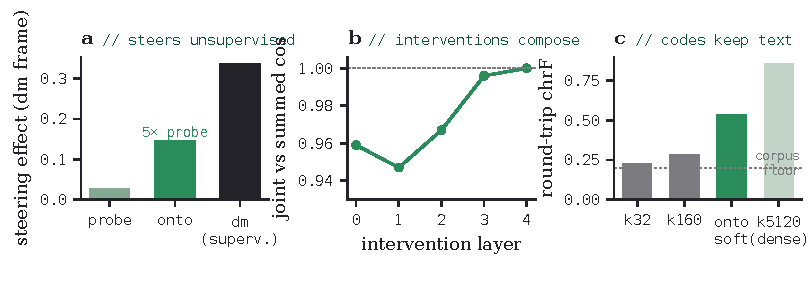
\includegraphics[width=\linewidth]{figures/fig-teaser.pdf}
\caption{The proposition, measured. Left: forcing classifications
moves decodes along the supervised difference-of-means direction
$0.43\times$ as far as supervised steering itself and $5\times$
further than probe directions, the strongest unsupervised arm tested
(Table~\ref{tab:steer-overlay}). Center: joint interventions point
where the summed single interventions point, exactly so in the final
layer (working notes). Right: the sparse SAE tier's codes lose most
text before any intervention is applied (round-trip chrF
$0.23$--$0.29$ against a $0.20$ corpus floor) while the Ontologizer's
soft code preserves it, so low-collateral steering is available only
to the soft architectures; the dense k5120 SAE preserves text but is
not a sparse steering code (working notes).}
\label{fig:teaser}
\end{figure}

\section{Assumptions}

This proposal assumes:
\begin{itemize}
	\item \textbf{Steering is inherent to the training objective.}
	The dictionary vectors must also be high quality steering vectors;
	interpretability and steering are treated as the same problem.
	\item \textbf{Weights are themselves interpretable} (for certain architectural choices).
	\item \textbf{Clustering rather than decomposition.} Representations
	are grouped into mutually contrastive categories rather than
	decomposed into independently firing features. The clustering framing
	is counterintuitive unless you arrive at it from Leiden-style
	community detection.
	\item \textbf{Categorical structure is imposed on features.}
	\item \textbf{Interpretability gets a cheap forward pass.}
	\item \textbf{Concepts compose linearly.} Concepts must be additive to be
	useful.
	\item \textbf{Dictionary learning is all you need}, in a nonstandard
	form: the dictionary forms a basis for the representation rather than
	a target.
	\item \textbf{Representations are not themselves quantized.} The
	learned dictionary serves as a basis for the representation rather
	than a discrete codebook; quantization comes from sharpening of
	classifications over that basis.
	\item \textbf{Interpreting a well trained model is the same problem
	as interpreting the data and training tasks.}
\end{itemize}

\subsection{Pivotal assumptions}
Two of these are pivotal: some version of the linear representation
hypothesis is true, and latent space is in some way ``natural''.

\subsection{Concerns}

\paragraph{Timelines could be too short}
We'll just have to go faster.

\paragraph{Contrastive classifiers might not be expressive enough}
This is what the reconstruction benchmarks are for. The preliminary
numbers (Section~\ref{sec:prelim}) put a price on the constraint; the
open question is whether steering quality justifies it.

\paragraph{Steering could push it too far off manifold}
This is an open problem in mechinterp. Diffusion steering is one
candidate to address it\cite{wagenmaker2025}.
If we can't solve the problem it still gives good data to test steering
methods. e.g.\ can we RL a model for high/low scores on a classification
and have it converge faster than paired steering or PCA vectors?
A first pass exists: a REINFORCE policy over steering directions on
frozen \texttt{resid\_nc\_hm}, rewarded by one classification's
quantile-normalized score at a matched intervention budget, converges
cleanly in the differentiable in-embedding tier, saturating within
roughly 40 steps at flat collateral (Figure~\ref{fig:rl}). Neither the
decode-cycle tier nor the convergence race against paired steering has
been run; the race is the test this paragraph proposes.

\begin{figure}[tp]\centering
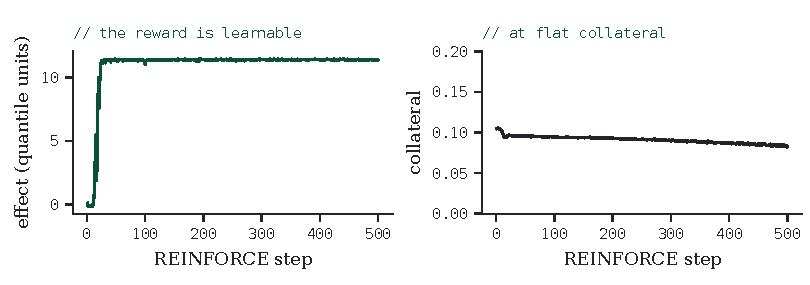
\includegraphics[width=\linewidth]{figures/fig-rl.pdf}
\caption{REINFORCE against a single frozen classification's
quantile-normalized score, in-embedding tier. The policy saturates the
reward within roughly 40 steps while collateral stays at its starting
level; a classification is a trainable objective.}
\label{fig:rl}
\end{figure}

\paragraph{Representations could be too soft/dense/high entropy}
This is highly correlated across all feature-based interp (SAEs,
transcoders, J-space). Dividing representations across orthogonal
categorical subspaces makes it possible to interpret the conceptual
basis vectors even if the representations are dense mixtures.

\paragraph{Ontofeatures could be too polysemantic}
Orthogonality \& categorical constraints give a theoretical inductive
bias to monosemanticity. As long as they have decent explanatory power
we can do eigendecomposition; polysemanticity decreases with parameter
count and we have more directions to increase parameters (in addition to
increasing width we can increase head size or stack more layers).
A first star sweep tests the scaling prediction at reduced training
(architecture and terms defined in Section~\ref{sec:arch}): seven
configurations around the shared $h{=}32$, $k{=}32$, $l{=}5$ shape,
varying one axis at a time, each trained 4 epochs (62k steps; the
retrain recipe's 24 epochs is 372k steps). No measured axis delivers
the predicted rise: head coherence shows no positive relation to
parameter count
(Spearman $+0.14$ for mean $z_{\cos}$, $-0.54$ for the fraction above
$z{=}2$), usage imbalance grows with size ($+0.86$), and the cleanest
per-axis trend runs opposite to the claim, coherence falling
monotonically as entries per head grow ($k{=}16/32/64$: mean $z_{\cos}$
$20.2/6.3/3.7$). One confound is recorded: the widest model ($h{=}64$)
has not converged at this budget (tail MSE $20\times$ the others), so
its collapse is not evidence (Figure~\ref{fig:scaling}). Seven points
at short training are weak evidence either way; full-length retrains
are the missing control.

\begin{figure}[tp]\centering
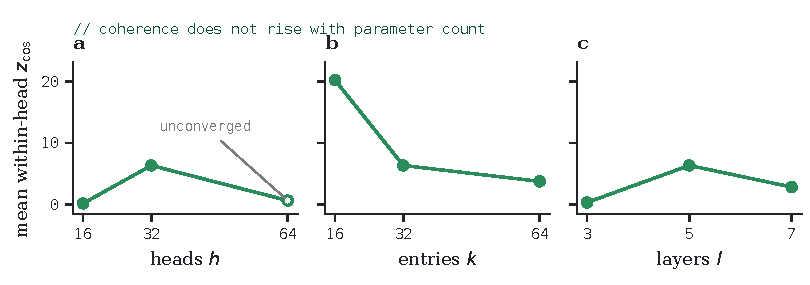
\includegraphics[width=\linewidth]{figures/fig-scaling.pdf}
\caption{Head coherence against each parameter axis of the star sweep,
all runs at 4 epochs (62k steps) of the retrain recipe's 24. No axis
delivers the predicted rise; the entries axis falls monotonically. The
open marker is the unconverged $h{=}64$ run.}
\label{fig:scaling}
\end{figure}

\paragraph{Interpreting ontofeatures could be otherwise intractable}
This would imply the universality hypothesis is false and is highly
correlated with intractability of other interpretability agendas.
Submodules could be interpretable even if features aren't.

\paragraph{Training could be intractable}
Sparsity trades against sample/compute efficiency; preliminary
experiments suggest we have less need for a sparsity constraint
(working notes).

\paragraph{Too many hyperparameters/too hyperparameter dependent}
This generally becomes less of an issue with scaling; preliminary
experiments show most changes to hyperparameters just change the rate of
convergence (working notes).

\paragraph{Doesn't converge in the limit}
Collapse in one layer would propagate down the stack. Candidate causes:
underparameterization, a really bad optimizer, bad initialization, a bad
loss term.

\paragraph{Not orthogonal in the limit}
$\mathrm{cossim}_h$ (Section~\ref{sec:loss}) penalises overlap between
heads but does not
guarantee disjoint support at convergence. The head geometry
(Figure~\ref{fig:head-simplex}) is built to make orthogonality the cheap
solution, not to force it.

\paragraph{Might not generalize out of distribution}
The same concern applies to every feature-based technique. Closed-form
interpretation of the dictionary is the mitigation: a statically
interpreted basis does not depend on the input distribution, though the
classifications over it do.

\paragraph{Inference too expensive}
Each layer adds $h \cdot k$ classifications per sample
(Section~\ref{sec:arch}), with $k$ small;
the code is computed without materializing a wide feature space. The
cost is the extra decoder passes for deep supervision during training.

\paragraph{Autointerp doesn't work on parameters/eigenfeatures}
In the preliminary experiments, parameter-space decodes of feature
directions failed as descriptions outright
(Section~\ref{sec:prelim-autointerp}). This is direct evidence against
the static-interpretability claim.

\section{Motivation}

\subsection{Threat Model}

\subsubsection{The ontology identification problem}
We can't yet reliably look inside a model and draw conclusions about its
goals or world model; interpretability has found a model's hidden
objective in a planted test~\cite{marks2025}.
This is a major limitation on almost all proposed alignment agendas,
because behavior alone cannot settle the question: a model can behave
differently when it believes it is being trained, and when that belief
reaches it through training documents rather than its prompt, the
difference can persist with no written reasoning to
inspect~\cite{greenblatt2024}. Only some models show such a
gap~\cite{sheshadri2025}, but that a good record under test need not
predict later behavior is an old argument~\cite[Ch.~8]{bostrom2014}.

\paragraph{Inner misalignment}
We don't currently know how to specify a robust goal for a model.
Because goal space is large, we should expect
goal misgeneralization as the default outcome.


\subsubsection{Limits of natural abstractions}
Networks trained on the same task can share an algorithm across
architectures while differing, even between random seeds, in which
features implement it: evidence for weak but not strong
universality~\cite{chughtai2023}. In language models, SAE features of a
Transformer and a Mamba trained on the same data match nearly as well as
those of two Transformer seeds~\cite{wang2024}.
This implies the existence of at least a weak version of
natural abstractions~\cite{lang2023},
which would be a very convenient shortcut for auditing a model.

Natural abstractions could be considered the set of concepts we could use to communicate with aliens. 
They should consistently emerge through unsupervised learning (in the limit given some constraints).
If any neural network is considered a fuzzy generalization of a finite state machine, 
natural abstractions are the latent states.

Unfortunately, the abstractions a model learns seem highly sensitive to choice of training data, and even to the random seed with the data fixed~\cite{chughtai2023}, and are thus not necessarily universal in the limit.
\footnote{The same applies to those that seem most natural to humans.}
Assuming that model capabilities will continue to primarily be driven by access to more data and more modalities, we cannot expect the abstractions learned by a weak model to remain robust in a more powerful model.

Even if we could fully characterise a model's state space in terms of natural abstractions,
that still doesn't mean we can reconstruct the latent FSM, 
as the transition rules can be arbitrarily complex.


\subsection{Theory of change}
Conditional on the underlying model of ontology being true, the
techniques proposed here would be a substantial interpretability
advance. The agenda also has a case for counterfactual impact: its
theoretical basis consists of nonobvious applications of obscure
techniques from niche fields of bioinformatics, and similar research
is unlikely to be done soon otherwise.

\subsubsection{What a solution would look like}
Mechinterp plausibly offers the best path to a robust alignment
solution despite criticisms.
The case rests on
\begin{enumerate}
    \item \textbf{decomposability} Mechinterp allows alignment to be
    broken into manageable subproblems.
    \item \textbf{parallelizability} Decomposable subproblems can be
    worked on independently.
    \item \textbf{robustness} Mechinterp offers direct causal
    explanations of model behavior.
\end{enumerate}
The most straightforward mechinterp alignment solutions are
\begin{enumerate}
    \item eliciting latent knowledge (ELK)
    Directly inferring a model's ontology.
    \label{it:elk}
    \item mechanistic anomaly detection (MAD)
    Detecting when a model has ``unusual'' thoughts.
    \label{it:mad}
\end{enumerate}
Both of these can be considered
ontology identification subproblems. MAD requires mapping between the model's activations and
the model's ontology. ELK requires mapping between the model's ontology
and human ontology. These are hard but not intractable problems.
Recently, developmental interpretability
(devinterp) techniques have enabled identification of ``developmental
stages'' corresponding to learning specific
tasks~\cite{hoogland2024developmental}. This is strong evidence that
learning consists primarily of the network
grokking~\cite{nanda2023progress} discrete concepts. While these results
are promising for MAD, locating these emergent capabilities in the
model's activations remains an open problem.

Interpretability glosses broadly as ``let humans understand AI''. Getting
AI to understand humans better scales badly: making the model smarter
leads to subtler and subtler issues with larger and larger effects.
Between the two sits scalable oversight, in which models help humans
supervise models: people working with an unreliable dialog assistant
already outperform both the assistant and themselves
alone~\cite{bowman2022}, and interpretability is one of the channels such
oversight can draw on. And what we're doing is not just
letting humans understand AI. Because an LLM reflects humanity from its
training data, high quality conceptual interpretability provides
machine-comprehensible mathematical representations of every concept
that humanity cares about. We work on interp for the usual
corrigibility reasons, and also because outer alignment needs a stable
place to attach values: a goal defined over one of a model's concepts
must keep pointing at that concept as the model's representations are
revised~\cite[Ch.~12]{bostrom2014}. The preliminary results measure a
small version of this problem: past the first layer, no head survives a
change of seed (Section~\ref{sec:prelim-seed}). This attacks both.

\subsubsection{Macro-scale strategy}
Broadly, the goals are to
\begin{enumerate}
  \item formalize the notion of a model's latent concept space
  \item distill a model's latent concept space
  \item enforce decomposability of latent concept space
  \item enforce robustness of existing concepts as the dimensionality of
  the latent concept space increases
\end{enumerate}
A prerequisite for all of these is the ability to express a
metaontology
which can identify latent concepts in activation space.



\section{Background}
Mechanistic interpretability currently can do supervised steering well
or unsupervised steering poorly. This has prompted the Google Deep Mind
interpretability team to pivot to a pragmatic steering
agenda\cite{gdmprogress2025}. Compared to unsupervised interpretability,
supervised steering is highly robust. However it can only distinguish
what the experimenter is looking for and does not account for the actual
computations performed by a model\cite{makelov2023}. The dominant
unsupervised paradigm is the sparse autoencoder (SAE). A model's hidden
state is approximated as a finite state machine consisting of discrete
features. The initial implementation used a $\relu$ activation and
sparsity loss\cite{bricken2023}, though more recent implementations have
used a $\topk$ activation function without a sparsity loss\cite{gao2024}.

\subsection{Common problems with SAEs}
The motivation is to decompile a model to a finite state machine (FSM).
The limitation is that such an FSM is only as interpretable as an
enumeration of all possible states.

\subsubsection{Features are not composable}
A persistent problem with SAEs is feature absorption\cite{chanin2025}.
Instead of representing an input as a composition of monosemantic
features, an SAE will often instead use a single separate feature. This
is a problem for interpretability, as we would like features to
generalize. One attempt to address this problem is Matryoshka
SAEs\cite{bussmann2025}, which use multiple layers to build a
hierarchical coarse-to-fine representation.

\subsubsection{Features are not causal}
Sparsity trades off against reconstruction fidelity. Using features for
steering often results in inconsistent, context-sensitive
behavior\cite{duan2026}.

\subsubsection{Features are not closed-form}
A major concern is how well an interpretability technique generalizes
out-of-distribution. Ideally we would like to infer behavior by looking
solely at model weights, which can be achieved with bilinear
MLPs\cite{pearce2025}.

\subsubsection{Forward passes are expensive}
Efficiency is also a problem. Although the sparsity constraint means
that only a handful of features are active for a given input, the
entire feature space needs to be computed for each sample.
Mixture-of-experts (MoE) SAE variants reduce compute costs by dividing
feature space between smaller submodules. Examples include Switch
SAEs\cite{mudide2025} and Tree SAEs\cite{cao2026}.

Less explored is the effect of the structure imposed by the MoEfied
architecture on the interpretability of feature space. A common approach
to scalably interpreting features is using an LLM to predict activations
from examples\cite{paulo2025}. With an unstructured feature space, it
quickly becomes intractable to interpret all permutations of features
this way. It is however possible to instead apply this technique to
expert routings. The MLPs of a transformer can themselves be converted
to an MoE architecture\cite{zhang2022}. Language models seem to organize
contrastive concepts into orthogonal simplices\cite{park2025}. This is
suggestive of MoEfication revealing latent contrastive steering vectors.
Imposing an orthogonality constraint has been shown to significantly
reduce feature absorption\cite{korznikov2025}.

Existing attempts to route activations to expert SAEs focus on routing
similar inputs to the same expert. Contrastive learning wants the
opposite: training on things at opposite ends of a shared axis. We don't
just want to find similar features, we want to find contrastive vectors
in feature space that correspond to what a model considers a natural
category.




\section{Methods}

\subsection{Architecture}
\label{sec:arch}
We propose a method that encodes samples as classifications mapped to
contrastive vectors. This directly constrains a model's representations,
and classifications can natively be used for steering.

The model (Figure~\ref{fig:onto-stack}) consists of $l$ $\dictenc$
layers writing into a shared residual accumulator, decoded by a single
linear map. Each layer (Figure~\ref{fig:dictenc}) is a classifier
followed by a dictionary. The classifier splits its input into $h$
independent \emph{assignments}, each a distribution over one head's $k$
\emph{entries}, and the dictionary maps each entry to an \emph{atom}.
Each layer writes the assignment-weighted sum of its atoms to the
accumulator; after each layer the accumulator is decoded and the residual
passed on, so layer $\ell$ receives $\mathbf{x} - \mathrm{dec}(\mathbf{r}_\ell)$,
where $\mathbf{r}_\ell$ holds the $\ell$ layers before it. Deep supervision
constrains every prefix of the stack to reconstruct the input.

Because entries within a head are mutually exclusive rather than
independent, each head is a contrastive set: a $k$-way classifier whose
entry swaps are steering moves. A between-head penalty is meant to push
each head onto its own coordinates of the dictionary space
(Figure~\ref{fig:head-simplex}); measured on the trained models, it did
not (Section~\ref{sec:disjoint}).

\begin{figure}[tp]
\centering
\resizebox{\linewidth}{!}{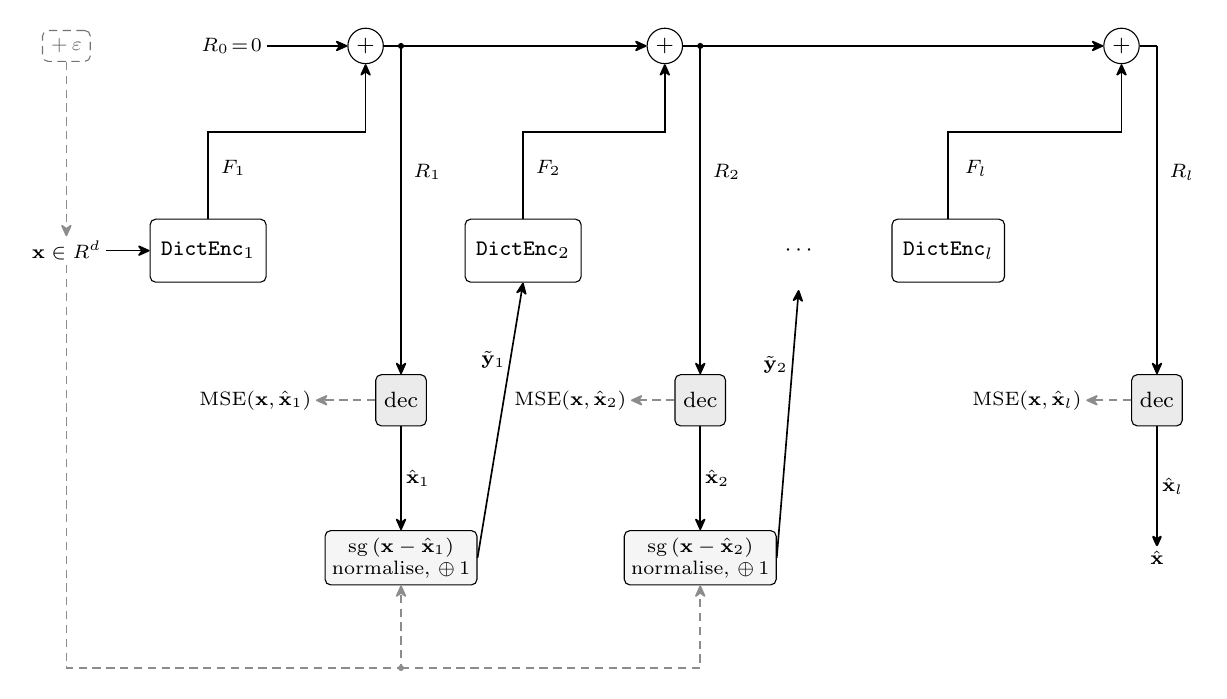
\begin{tikzpicture}[
    font=\footnotesize,
    >={Stealth[round,length=1.8mm,width=1.6mm]},
    blk/.style={draw, rounded corners=2pt, align=center,
                minimum height=8mm, inner xsep=4pt},
    hook/.style={draw, rounded corners=2pt, densely dashed, align=center,
                 inner sep=3pt, font=\scriptsize, black!55},
    dec/.style={draw, rounded corners=2pt, fill=black!8,
                minimum height=6.5mm, inner xsep=3pt},
    cond/.style={draw, rounded corners=2pt, fill=black!4, align=center,
                 inner sep=2.5pt, font=\scriptsize},
    add/.style={draw, circle, minimum size=4.5mm, inner sep=0pt},
    lab/.style={inner sep=1.5pt, font=\scriptsize},
    sig/.style={->, semithick},
    aux/.style={->, densely dashed, semithick, black!45},
  ]

  %% ---- layer row --------------------------------------------------
  \node[lab] (x)  at (-1.5,0) {$\mathbf{x}\in\mathbb{R}^{d}$};
  \node[blk] (D0) at ( 0.3,0) {$\mathtt{DictEnc}_1$};
  \node[blk] (D1) at ( 4.3,0) {$\mathtt{DictEnc}_2$};
  \node      (Dd) at ( 7.8,0) {$\cdots$};
  \node[blk] (DL) at ( 9.7,0) {$\mathtt{DictEnc}_{l}$};

  \draw[sig] (x) -- (D0);

  \node[hook] (noise) at (-1.5,2.6) {$+\,\varepsilon$};
  \draw[aux] (noise) -- (x);

  %% ---- residual accumulator (top rail, y = 2.6) --------------------
  \node[add] (A0) at ( 2.3,2.6) {$+$};
  \node[add] (A1) at ( 6.1,2.6) {$+$};
  \node[add] (AL) at (11.9,2.6) {$+$};

  \node[lab] (R0) at (0.6,2.6) {$R_0\!=\!0$};
  \draw[sig]      (R0) -- (A0);
  \draw[sig]      (A0) -- (A1);
  \draw[sig]      (A1) -- (AL);
  \draw[semithick] (AL) -- (12.35,2.6);

  %\node[lab] at (8.9,3.05) {$R\in\mathbb{R}^{e}$: residual accumulator};

  %% ---- per-layer contributions F_i (enter from below) --------------
  \draw[sig] (D0.north) -- ++(0,1.1) -| (A0.south);
  \draw[sig] (D1.north) -- ++(0,1.1) -| (A1.south);
  \draw[sig] (DL.north) -- ++(0,1.1) -| (AL.south);
  \node[lab] at (0.62,1.05) {$F_1$};
  \node[lab] at (4.62,1.05) {$F_2$};
  \node[lab] at (10.05,1.05) {$F_{l}$};

  %% ---- shared decoder, one decode per prefix -----------------------
  \node[dec] (Y1) at ( 2.75,-1.9) {$\mathrm{dec}$};
  \node[dec] (Y2) at ( 6.55,-1.9) {$\mathrm{dec}$};
  \node[dec] (YL) at (12.35,-1.9) {$\mathrm{dec}$};

  \draw[sig] ( 2.75,2.6) -- (Y1.north);
  \draw[sig] ( 6.55,2.6) -- (Y2.north);
  \draw[sig] (12.35,2.6) -- (YL.north);
  \fill ( 2.75,2.6) circle (1.1pt);
  \fill ( 6.55,2.6) circle (1.1pt);

  \node[lab,anchor=west] at ( 2.85,1.0) {$R_1$};
  \node[lab,anchor=west] at ( 6.65,1.0) {$R_2$};
  \node[lab,anchor=west] at (12.45,1.0) {$R_l$};

  %% ---- deep supervision --------------------------------------------
  \node[lab] (L1) at ( 0.9,-1.9) {$\mathrm{MSE}(\mathbf{x},\hat{\mathbf{x}}_1)$};
  \node[lab] (L2) at ( 4.9,-1.9) {$\mathrm{MSE}(\mathbf{x},\hat{\mathbf{x}}_2)$};
  \node[lab] (LL) at (10.7,-1.9) {$\mathrm{MSE}(\mathbf{x},\hat{\mathbf{x}}_l)$};
  \draw[aux] (Y1.west) -- (L1);
  \draw[aux] (Y2.west) -- (L2);
  \draw[aux] (YL.west) -- (LL);

  %% ---- residual forwarding ------------------------------------------
  \node[cond] (C1) at (2.75,-3.9)
  {$\mathrm{sg}\,(\mathbf{x}-\hat{\mathbf{x}}_1)$\\ normalise, $\oplus\,1$};
  \node[cond] (C2) at (6.55,-3.9)
  {$\mathrm{sg}\,(\mathbf{x}-\hat{\mathbf{x}}_2)$\\ normalise, $\oplus\,1$};
  \draw[sig] (Y1) -- node[right,lab]{$\hat{\mathbf{x}}_1$} (C1);
  \draw[sig] (Y2) -- node[right,lab]{$\hat{\mathbf{x}}_2$} (C2);

  \draw[sig] (C1.east) -- node[left,lab,pos=0.72]{$\tilde{\mathbf{y}}_1$} (D1.south);
  \draw[sig] (C2.east) -- node[left,lab,pos=0.72]{$\tilde{\mathbf{y}}_2$} (7.8,-0.5);

  %% ---- model output --------------------------------------------------
  \node[lab] (out) at (12.35,-3.9) {$\hat{\mathbf{x}}$};
  \draw[sig,thick] (YL) -- node[right,lab]{$\hat{\mathbf{x}}_l$} (out);

  %% ---- x broadcast to every conditioning step -------------------------
  \draw[aux] (x.south) -- (-1.5,-5.3) -- (2.75,-5.3) -- (C1.south);
  \draw[aux] (2.75,-5.3) -- (6.55,-5.3) -- (C2.south);
  \fill[black!45] (2.75,-5.3) circle (1.1pt);

\end{tikzpicture}

}
\caption[\texttt{Ontologizer} architecture]{\textbf{\texttt{Ontologizer} architecture.}
	An \texttt{Ontologizer} consists of $l$ stacked \texttt{DictEnc} layers.
	Each returns a pooled feature vector $\mathbf{f}'_\ell\in\mathbb{R}^{e}$,
	which is written, scaled by its input's gain $g_\ell$, to a residual
	accumulator $\mathbf{r}$.
	Layers are indexed $\ell = 0, \dots, l-1$ and accumulator states by the
	number of layers applied: $\mathbf{r}_0 := \mathbf{0}$ and
	$\mathbf{r}_{\ell+1} = \mathbf{r}_\ell + g_\ell\,\mathbf{f}'_\ell$, so
	layer $\ell$ reads state $\ell$ and writes state $\ell+1$; a stop-gradient
	variant ($\mathrm{sg}$ on $\mathbf{r}_\ell$, available but off in every model
	reported here) would prevent gradient communication between layers.
	$\mathrm{dec}$ is a linear decoder with shape $\mathbb{R}^{d \times e}$,
	shared by all layers.
	Deep supervision gives a coarse-to-fine representation where
	the component encoded by previous layers is inaccessible to later layers.
	After $\ell$ layers, $\hat{\mathbf{x}}_\ell = \mathrm{dec}(\mathbf{r}_\ell)$, and
	the component left unexplained is
	$\mathbf{y}_\ell = \mathbf{x} - \hat{\mathbf{x}}_\ell$, so $\mathbf{y}_0 = \mathbf{x}$.
	Layer $\ell$ classifies the shape of its input,
	$\mathbf{u}_\ell
	  = \mathbf{y}_\ell / \mathrm{L2}(\mathbf{y}_\ell) \oplus [1]$, and scales
	what it writes by the gain $g_\ell = \mathrm{L2}(\mathbf{y}_\ell)$.
	Normalizing prevents exploding gradients from repeated
	application of bilinear layers, each of which scales its input by
	$\lVert\cdot\rVert^{2}$; the constant coordinate keeps the sign of
	$\mathbf{y}_\ell$, which the bilinear form would otherwise lose.
	$\mathrm{MSE}(\mathbf{x},\hat{\mathbf{x}}_\ell)$ is computed separately for
	each prefix $\ell = 1, \dots, l$. The input-noise hook drawn on $\mathbf{x}$ is disabled in
	every model reported here.
}
\label{fig:onto-stack}
\end{figure}

\subsubsection{Classifier}
\label{sec:bilinear}
Each $\dictenc$'s classifier is a multihead bilinear map
($\bilinearblock$) with weights
$[\mathsf{W}, \mathsf{V}] \in \mathbb{R}^{2 \times h \times k \times d}$
($d+1$ with the constant coordinate of Equation~\ref{eq:y_norm}). It
reads the shape $\mathbf{u}_\ell$ of the layer's input (the residual left
by the layers before it, or $\mathbf{x}$ at layer 0), written $\mathbf{x}$
below for a generic input, and returns logits $K \in \mathbb{R}^{h \times k}$,
\begin{equation}
	\bilinearblock([\mathsf{W},\mathsf{V}],\mathbf{x}) :=
	\left(\sum^{d}_{q=1}W_{\cdot\cdot q}\,x_q\right)
	 \odot \left(\sum^{d}_{q=1}V_{\cdot\cdot q}\,x_q\right).
	 \label{eq:bilinearblock}
\end{equation}
Each logit is a quadratic form in $\mathbf{x}$, so a classifier admits
closed-form eigendecomposition in the manner of bilinear
MLPs\cite{pearce2025}.

\begin{figure}[tp]
\centering
\resizebox{\linewidth}{!}{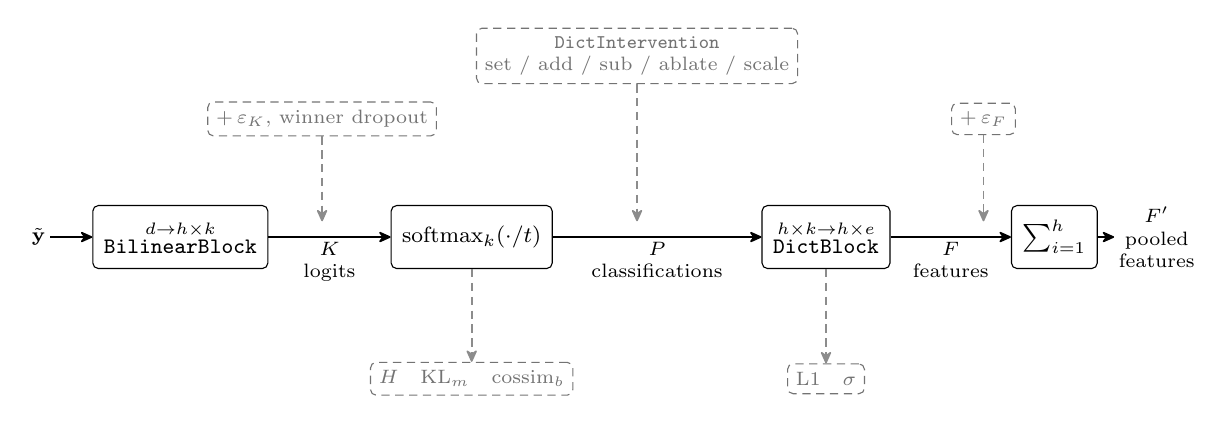
\begin{tikzpicture}[
    font=\footnotesize,
    >={Stealth[round,length=1.8mm,width=1.6mm]},
    blk/.style={draw, rounded corners=2pt, align=center,
                minimum height=8mm, inner xsep=4pt},
    hook/.style={draw, rounded corners=2pt, densely dashed, align=center,
                 inner sep=3pt, font=\scriptsize, black!55},
    lab/.style={inner sep=1.5pt, font=\scriptsize, align=center},
    sig/.style={->, semithick, align=center},
    aux/.style={->, densely dashed, semithick, black!45},
  ]

  %% ---- main chain ----------------------------------------------------
  \node[lab] (E)  at (-0.6,0) {$\tilde{\mathbf{y}}$};
  \node[blk] (CL) at ( 1.2,0) {$\bilinearblock^{d \to h \times k}$};
  \node[blk] (SM) at ( 4.9,0) {$\mathrm{softmax}_k(\cdot/t)$};
  \node[blk] (DB) at ( 9.4,0) {$\dictblock^{h \times k \to h \times e}$};
  \node[blk] (SU) at (12.3,0) {$\sum^{h}_{i=1}$};
  \node[lab] (F)  at (13.6,0) {$F'$\\ pooled\\ features};

  \draw[sig] (E)  -- (CL);
  \draw[sig] (CL) -- node[below,lab]{$K$\\ logits}   (SM);
  \draw[sig] (SM) -- node[below,lab]{$P$\\ classifications}   (DB);
  \draw[sig] (DB) -- node[below,lab]{$F$\\ features} (SU);
  \draw[sig] (SU) -- (F);

  %% ---- training-time hooks and the intervention interface (above) ----
  \node[hook] (nk) at (3.0,1.5) {$+\,\varepsilon_K$,\ winner dropout};
  \node[hook] (iv) at (7.0,2.3) {\texttt{DictIntervention}\\
                                 set / add / sub / ablate / scale};
  \node[hook] (nf) at (11.4,1.5) {$+\,\varepsilon_F$};
  \draw[aux] (nk) -- (3.0,0.20);
  \draw[aux] (iv) -- (7.0,0.20);
  \draw[aux] (nf) -- (11.4,0.20);

  %% ---- where each regulariser attaches (below) -----------------------
  \node[hook] (lp) at (4.9,-1.8)
    {$H$\quad $\mathrm{KL}_m$\quad $\mathrm{cossim}_b$};
  \node[hook] (lf) at (9.4,-1.8)
    {$\mathrm{L1}$\quad $\sigma$};
  \draw[aux] (SM.south) -- (lp);
  \draw[aux] (DB.south) -- (lf);

\end{tikzpicture}

}
\caption[\texttt{DictEnc} architecture]{\textbf{\texttt{DictEnc} architecture.}
	Dashed lines above indicate perturbations to the data,
	including noising and causal interventions.
	Dashed lines below indicate statistics used as tuneable auxiliary loss
	functions. Each \texttt{DictEnc} consists of a multihead bilinear
	classifier (§\ref{sec:bilinear}) and a multihead dictionary
	(§\ref{sec:dict}). Noise $\varepsilon_K$ and $\varepsilon_F$ and winner
	dropout regularize training (§\ref{sec:noise}).
	Assignments $P$ are $\mathrm{softmax}_{k}(K/t)$, or its straight-through
	argmax (§\ref{sec:labels}); interventions act on $P$. From $P$ we
	collect per-sample entropy $H$, between-sample similarity
	$\mathrm{cossim}_b$ and batch-mean entropy $\mathrm{KL}_m$
	(Equations~\ref{eq:entropy}--\ref{eq:KL}). A $\dictblock$ maps
	$P \in \mathbb{R}^{h \times k}$ to features
	$F \in \mathbb{R}^{h \times e}$ (Equation~\ref{eq:dictblock}); from $P$
	and the atoms we collect the support overlap $\omega$
	(Equation~\ref{eq:support}), and from $F$ the sparsity penalty
	$\mathrm{L1}$. $F$ is summed over heads to give pooled
	features $\mathbf{f}' \in \mathbb{R}^{e}$, which are added to the
	accumulator $\mathbf{r}$.
}
\label{fig:dictenc}
\end{figure}

\subsubsection{Assignments and selection}
\label{sec:labels}
Soft assignments are $P = \mathrm{softmax}_{k}(K/t)$, where the
temperature $t$ is annealed to sharpen them. A soft code's argmax is
not, however, what the model decodes: Section~\ref{sec:prelim-pareto}
finds the softmax model's discrete reading far from its embedding. The
\emph{straight-through} selection rule makes the discrete code the model:
the forward pass selects the one-hot argmax, and the backward pass uses
$\mathrm{softmax}(K/t)$ as its surrogate gradient\cite{bengio2013}. A
hard code transmits exactly $l\,h\log_2 k$ bits and no continuous
coefficients.

From the assignments $P_n$ of each sample $n$ we collect per-sample
entropy, in bits,
\begin{equation}
	\mathrm{entropy}_k(P)_i :=
	-\sum^{k}_{j=1}p_{ij}\log_2 p_{ij},
	\qquad
	H := \mathbb{E}_{n}\,\mathbb{E}_{i}\!\left[
	\mathrm{entropy}_k(P_n)_i\right],
	\label{eq:entropy}
\end{equation}
between-sample similarity, the mean absolute cosine of the per-head
features over pairs of samples, evaluated through each head's dictionary
Gram $G_i = \lvert D_{i}\rvert \lvert D_{i}\rvert^{\top}$,
\begin{equation}
	\mathrm{cossim}_b(\mathsf{P}) :=
	\mathbb{E}_{n,n'}\left[\left\lvert
	\frac{\langle \mathbf{f}_{n}, \mathbf{f}_{n'}\rangle}
	     {\lVert \mathbf{f}_{n}\rVert \lVert \mathbf{f}_{n'}\rVert}
	\right\rvert\right],
	\qquad
	\langle \mathbf{f}_{n}, \mathbf{f}_{n'}\rangle
	= \sum^{h}_{i=1}\mathbf{p}_{ni}^{\top}G_{i}\,\mathbf{p}_{n'i},
	\label{eq:cossim_b}
\end{equation}
and the divergence of the batch-mean assignment from uniform,
\begin{equation}
	\mathrm{KL}_m(\mathsf{P}) := \mathbb{E}_{i}\!\left[\log_2 k -
	\mathrm{entropy}_k\!\left(\mathbb{E}_n[P_n]\right)_i\right].
	\label{eq:KL}
\end{equation}
$\mathrm{KL}_m$ anchors each head's mean assignment to uniform, which
keeps every entry in use.

\subsubsection{Dictionary}
\label{sec:dict}
A $\dictblock$ with weights $\mathsf{D} \in \mathbb{R}^{h \times k \times e}$
maps assignments to per-head features $F \in \mathbb{R}^{h \times e}$,
whose row $\mathbf{f}_i$ is head $i$'s output,
\begin{equation}
	\mathbf{f}_i :=
	\sum^{k}_{j=1} p_{ij}\,\mathbf{a}_{ij},
	\qquad
	\mathbf{a}_{ij} := \lvert \mathsf{D}_{ij\cdot}\rvert .
	\label{eq:dictblock}
\end{equation}
Atoms are non-negative and assignments lie on the simplex, so features
are strictly additive and each head's output lies in the convex hull of
its atoms (Figure~\ref{fig:head-simplex}).

\begin{figure}[tp]
\centering
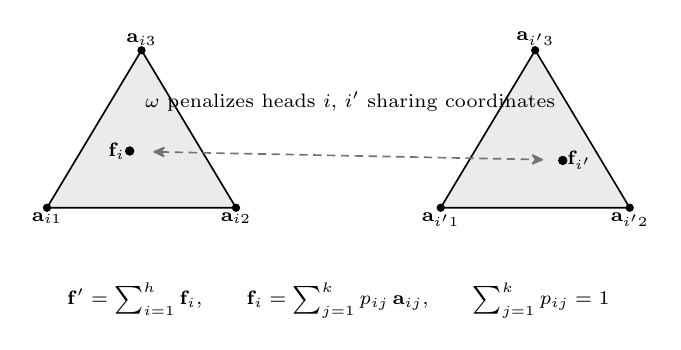
\begin{tikzpicture}[
    font=\footnotesize,
    >={Stealth[round,length=1.8mm,width=1.6mm]},
    lab/.style={inner sep=1.5pt, font=\scriptsize},
  ]
  %% ---- head i --------------------------------------------------------
  \fill[black!8]   (0,0) -- (2.4,0) -- (1.2,2.0) -- cycle;
  \draw[semithick] (0,0) -- (2.4,0) -- (1.2,2.0) -- cycle;
  \fill (0,0)     circle (1.5pt) node[below,lab]{$\mathbf{a}_{i1}$};
  \fill (2.4,0)   circle (1.5pt) node[below,lab]{$\mathbf{a}_{i2}$};
  \fill (1.2,2.0) circle (1.5pt) node[above,lab]{$\mathbf{a}_{i3}$};
  \fill (1.05,0.72) circle (1.7pt) node[left,lab]{$\mathbf{f}_i$};

  %% ---- head i' ------------------------------------------------------
  \fill[black!8]   (5.0,0) -- (7.4,0) -- (6.2,2.0) -- cycle;
  \draw[semithick] (5.0,0) -- (7.4,0) -- (6.2,2.0) -- cycle;
  \fill (5.0,0)   circle (1.5pt) node[below,lab]{$\mathbf{a}_{i'1}$};
  \fill (7.4,0)   circle (1.5pt) node[below,lab]{$\mathbf{a}_{i'2}$};
  \fill (6.2,2.0) circle (1.5pt) node[above,lab]{$\mathbf{a}_{i'3}$};
  \fill (6.55,0.60) circle (1.7pt) node[right,lab]{$\mathbf{f}_{i'}$};

  \draw[<->, densely dashed, semithick, black!55] (1.35,0.71) -- (6.30,0.61);
  \node[lab] at (3.85,1.35)
    {$\omega$ penalizes heads $i$, $i'$ sharing coordinates};

  \node[lab, anchor=north, align=center] at (3.7,-0.9)
  {$\mathbf{f}'=\sum^h_{i=1} \mathbf{f}_i$,\qquad
  $\mathbf{f}_i=\sum^k_{j=1} p_{ij}\,\mathbf{a}_{ij}$,\qquad $\sum^k_{j=1} p_{ij}=1$};
\end{tikzpicture}


\caption[Per-head geometry]{\texttt{DictBlock} \textbf{head geometry} for $h{=}2$; $k{=}3$.
	The output space of a head $i$ is a simplex with its atoms
	$\mathbf{a}_{ij}$, the rows of $\lvert D_i\rvert$, as vertices. The assignment $P$ is a soft
	choice among mutually contrastive categories rather than a set of
	independently firing features, and because $p_{ij} \in [0,1]$ the
	output lies within the convex hull of the head's atoms.
	Because $\lvert \mathsf{D}\rvert\geq0$ and $P\geq0$, $F\geq0$, so
	$\cos(\mathbf{f}_i, \mathbf{f}_{i'}) \in [0,1]$, and driving the support overlap $\omega$
	to zero asks the heads to partition the coordinates of $\mathbb{R}^e$
	between them (§\ref{sec:disjoint}).
}
\label{fig:head-simplex}
\end{figure}

\paragraph{Disjoint support}
\label{sec:disjoint}
For non-negative vectors the inner product is a sum of non-negative
terms, so it vanishes exactly when the supports are disjoint,
\begin{equation}
	\langle \mathbf{u},\mathbf{v}\rangle = 0
	\iff
	\mathrm{supp}(\mathbf{u}) \cap \mathrm{supp}(\mathbf{v}) = \emptyset .
	\label{eq:disjoint}
\end{equation}
Between heads, then, orthogonality is not a rotation constraint but a
support partition. The support overlap compares heads' usage-weighted
coordinate profiles,
\begin{equation}
	\boldsymbol{\pi}_i := \sum^{k}_{j=1} \bar{p}_{ij}\,
	\lvert \mathbf{a}_{ij}\rvert,
	\qquad
	\omega := \mathbb{E}_{i \neq i'}\,
	\frac{\langle \boldsymbol{\pi}_i, \boldsymbol{\pi}_{i'}\rangle}
	     {\lVert \boldsymbol{\pi}_i\rVert \lVert \boldsymbol{\pi}_{i'}\rVert},
	\qquad
	\bar{\mathbf{p}}_i := \mathbb{E}_{n}\,[\mathbf{p}_{ni}],
	\label{eq:support}
\end{equation}
and is zero exactly when no two heads share a coordinate. Because a
softmax gives every entry positive weight, a single sample on which two
heads are orthogonal forces every pair of their atoms to be disjoint:
the partition is a property of $\mathsf{D}$, holding for all inputs,
which is the premise a static reading of the dictionary needs.
Under $\mathtt{ConcatDictBlock}$ heads write disjoint slices by
construction and $\omega$ is identically zero.

Two orthogonalities are in play. Disjoint support assigns each head a
block of coordinates; \emph{within} a head the $k$ atoms are contrastive
alternatives spread apart inside that block, which
Section~\ref{sec:prelim-orth} measures. Neither is guaranteed at
convergence: $\omega$ is a penalty, and the geometry makes a support
partition the cheap solution rather than forcing one. Measured, the
within-head orthogonality holds and the between-head partition does not
form (Section~\ref{sec:prelim-orth}).

\subsubsection{Decoder}
\label{sec:decoder}
Each layer's pooled output $\mathbf{f}'_\ell = \sum_{i=1}^{h}\tilde{\mathbf{f}}_{i}$ is scaled
by its input's gain $g_\ell$ and added to the accumulator, whose state
after $\ell$ layers a single unbiased linear map shared by all layers
decodes,
\begin{equation}
	\mathbf{r}_\ell = \sum_{\ell'=0}^{\ell-1} g_{\ell'}\,\mathbf{f}'_{\ell'},
	\qquad
	\hat{\mathbf{x}}_\ell = W_{\mathrm{dec}}\mathbf{r}_\ell,
	\qquad
	W_{\mathrm{dec}} \in \mathbb{R}^{d \times e}.
	\label{eq:dec}
\end{equation}
The residual $\mathbf{y}_\ell$, layer $\ell$'s input, is stop-gradiented,
so that lower layers cannot write a communication code into it instead
of reducing it, and split into a gain and a shape $\mathbf{u}_\ell$, its
unit direction with a constant coordinate appended, which is what layer
$\ell$ classifies:
\begin{equation}
	\mathbf{y}_\ell = \mathrm{sg}\!\left[\mathbf{x} - \hat{\mathbf{x}}_\ell\right],
	\qquad
	\mathbf{u}_\ell =
	\frac{\mathbf{y}_\ell}{\mathrm{L2}(\mathbf{y}_\ell) + \epsilon} \oplus [1],
	\qquad
	g_{\ell} := \mathrm{sg}\!\left[\mathrm{L2}(\mathbf{y}_\ell)\right].
	\label{eq:y_norm}
\end{equation}
The empty sum makes $\mathbf{r}_0 = \mathbf{0}$, so $\mathbf{y}_0 = \mathbf{x}$:
layer 0 classifies the input itself.
Under \texttt{resid\_gain} each layer classifies the direction of what it
corrects, and the gain carries the magnitude it cannot see; without it
$g_\ell = 1$.

\paragraph{Direct atoms and fibers.}
Two variants change what an entry writes. With \emph{direct atoms} the
dictionary is signed and lives in the output space itself, with no
decoder, so every atom is literally a steering direction. With
\emph{fibers} each entry carries a rank-$r$ local basis, and each head
reads $r$ coordinates from its input, so a hard code becomes a discrete
base point plus a continuous correction within that entry's fiber;
training the fibers after freezing the base keeps the discrete code
exactly what it was.

\subsubsection{Noise and dropout}
\label{sec:noise}
Classifier logits take Gaussian noise $\varepsilon_K$, relative to the
logit scale under a hard forward; features take noise $\varepsilon_F$
proportional to each feature's batch standard deviation, stop-gradiented
so the model cannot evade it by shrinking variance. Winner dropout sets a
head's argmax logit to $-\infty$ with probability $p_{\mathrm{drop}}$.

\subsection{Training}
\label{sec:training}

\subsubsection{Embedding model}
\label{sec:sonar}
We embed texts using SONAR\cite{sonar}, a multimodal and
language-agnostic sentence embedding model. SONAR embeddings correspond
to entire texts rather than tokens, are paired with a decoder, and encode
language independently of content, which allows steering fidelity to be
validated against a ground truth. Large Concept
Models\cite{lcmteam2024largeconceptmodelslanguage} generate directly in
SONAR space, which makes it a natural substrate for steering
experiments. GPT-2 small's residual stream\cite{radford2019} is a second
substrate, where sparse dictionary learning is known to work and the
reconstruction can be spliced back into the model.

\subsubsection{Loss function}
\label{sec:loss}
Reconstruction is trained with a whitened MSE, $\mathbf{w}$ being the
per-dimension inverse variance normalized to mean one,
\begin{equation}
	\mathrm{MSE}(X,\hat{X}) := \frac{1}{bd}\sum^{b}_{n=1}\sum^{d}_{q=1}
	w_q\left(\hat{x}_{nq} - x_{nq}\right)^2,
	\label{eq:mse}
\end{equation}
under deep supervision: it is computed at every prefix
$\hat{X}_\ell$, $\ell = 1, \dots, l$, and averaged, so each layer must explain
what earlier layers left unexplained. The auxiliary statistics are weighted
and summed over layers,
\begin{equation}
	L := \frac{1}{l}\sum^{l}_{\ell=1}\mathrm{MSE}(X,\hat{X}_\ell)
	+ \sum^{l-1}_{\ell=0}\mathbf{s}\cdot\boldsymbol{\psi}_\ell,
	\qquad
	\boldsymbol{\psi}_\ell := \big[\, \mathrm{L1} \;\; \mathrm{cossim}_b \;\;
	\mathrm{KL}_m \;\; \omega \,\big]^{\top}_\ell,
	\label{eq:loss_total}
\end{equation}
with $\mathrm{L1}$ the batch mean of each sample's feature norm. In
practice $\mathrm{cossim}_b$ also minimizes $H$, which therefore carries
no weight. Every model reported here trained before $\omega$ existed, with
its predecessor in that slot: the mean cosine between heads' features
within a sample, which for non-negative features stands in for the same
disjointness.

\subsection{Evaluation}
\label{sec:eval}
Evaluation runs against $\topk$ SAEs\cite{gao2024} trained on the same
cached embeddings under the same whitened objective, scored by whitened
fraction of variance unexplained ($\mathrm{FVU}_w$) on a held-out tail.
A structural-ablation ladder of SAE variants adds one Ontologizer
commitment at a time; two of its rungs, which add per-head competition
over a shared decoder, are one-layer Ontologizers with linear
classifiers (\texttt{g160top1} with hard selection, \texttt{g160softmax}
with softmax) and are reported as simplified variants rather than
baselines. The headline instruments are reconstruction against code
capacity and its rate-distortion floor; the semantic coherence of a
head's decoded atoms against size-matched nulls; steering scored in
embedding space (whether a step realizes the target entry, and what
share of other heads it disturbs, against a random step of the same
length); additivity of paired interventions; cross-seed head matching
by partition and by contribution; and blinded auto-interpretability.
AxBench\cite{wu2025axbenchsteeringllmssimple} found that simple
supervised baselines beat SAEs at steering, and the steering comparison
is built to face that result.

\section{Preliminary results}
\label{sec:prelim}
The evaluation is in progress. Results so far are mixed. The full
methodology and numbers are in the working
notes\footnote{K.~Wiechecki, \emph{Dictionary learning as unsupervised
steering-vector generation: Ontologizers vs.\ sparse autoencoders on
SONAR sentence embeddings}, working notes, in preparation; distributed
with this proposal.}; the headlines are summarized here. Two models
recur throughout and are named once now. The notes' reference model,
\texttt{resid\_nc} (372{,}600 steps), is the model behind the notes'
tables, including Tables~\ref{tab:prelim-pareto}
and~\ref{tab:prelim-headcoh}. Its sibling \texttt{resid\_nc\_hm} is
the same configuration plus the batch mean-entropy bonus the notes
propose as the freeze fix, trained to 4.38M steps; the new experiments
reported here use its final checkpoint unless stated otherwise.

The notes carry one caveat about the reference: ``layer 4 froze 22/32
heads late in temperature annealing and is mildly harmful.'' A
diagnostic over both training histories (frozen: top classification
share ${\geq}0.95$ and churn ${\leq}0.02$) bears the caveat out and
locates the fix (Figure~\ref{fig:freeze}). In \texttt{resid\_nc}, the
top layer (layer 4 of 0--4) begins freezing near step 190k, well after
the anneal, reaches 27 of 32 by step 210k and 28 at its peak, and is
still frozen at the last checkpoint; the count differs from the notes'
22 under this criterion, the layer and the persistence do not. In
\texttt{resid\_nc\_hm} the late freeze never occurs: what remains is
an early annealing transient (22 of 32 at layer 1 of 0--4 at step 10k,
with 16, 11, and 4 of 32 at layers 2, 3, and 0) that recovers
completely by step 30k, leaving the final checkpoint unfrozen
everywhere. The mean-entropy bonus does what the notes proposed it
for.

\begin{figure}[tp]\centering
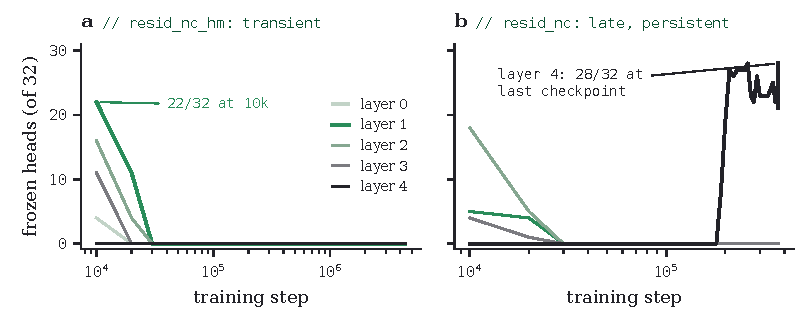
\includegraphics[width=\linewidth]{figures/fig-freeze.pdf}
\caption{Frozen heads per layer over training (frozen: top
classification share ${\geq}0.95$, churn ${\leq}0.02$). Left:
\texttt{resid\_nc\_hm}, with the mean-entropy bonus, has only an early
annealing transient, peaking at 22/32 in layer 1 at step 10k and
recovering to zero everywhere by step 30k. Right: \texttt{resid\_nc},
the notes' reference, carries the caveat: a post-anneal layer-4 freeze
from ${\sim}$190k that persists through its last checkpoint.}
\label{fig:freeze}
\end{figure}

Four retrains of the \texttt{resid\_nc\_hm} configuration, a
zero-change control and three single-knob variants (372k steps each),
close the question of what drives the remaining transient. The control
reproduces it head-for-head (22/32 at layer 1 at step 10k, zero
everywhere by 30k) and shows no late freeze over its horizon.
Stretching the temperature anneal from 50k to 150k steps attenuates
and spreads the transient (peak 14/32 at layer 1 at step 30k, clear by
50k); raising winner dropout from $0.1$ to $0.25$ tracks the control
to within two heads at the peak, and holding the classification-noise
floor at its starting value changes nothing at all
(Figure~\ref{fig:variants}). The transient belongs to the temperature
schedule alone, and every retrain ends unfrozen everywhere.

\begin{figure}[tp]\centering
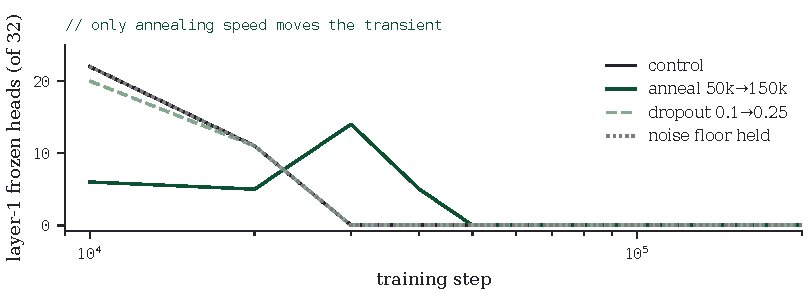
\includegraphics[width=\linewidth]{figures/fig-variants.pdf}
\caption{The early transient under the four retrains, layer-1 frozen
count. The noise-floor variant overlaps the control exactly and the
dropout variant tracks it to within two heads at the peak; only
stretching the temperature anneal moves the curve, trading peak height
for duration.}
\label{fig:variants}
\end{figure}

\subsection{Reconstruction quality}
Contrast-set structure is expensive. The plain-SAE frontier dominates
the Ontologizer's deviation code at every capacity tested
(Table~\ref{tab:prelim-pareto}), and the grouped-simplex constraint
alone costs roughly $40\times$ in weighted fraction of variance
unexplained. Here $\mathrm{FVU}_w$ is whitened MSE over the whitened
variance of a constant predictor, and the deviation code is a per-head
top-$m$ truncation around the measured mean classification
$\mathbb{E}[p]$. The train/eval asymmetry carries over from the notes: the
Ontologizer trained on the full cache including the evaluation tail,
while the SAEs excluded it; a fresh-encoded evaluation set is blocked
on a data source (Section~\ref{sec:future-completing}).

\begin{table}[tp]\centering\small
\begin{tabular}{@{}lrrr@{}}
\toprule
point & coeffs & index bits & $\mathrm{FVU}_w$ \\
\midrule
onto $m{=}0$ ($\mathbb{E}[p]$ origin) & 0 & 0 & 1.001 \\
onto hard (argmax)                  & 0 & 800 & 17.34 \\
sae k32 tier ($m{=}5120/11264$, incl.\ p5, s43) & 32 & $\sim$400 & 0.494--0.509 \\
sae k32 bilinear                    & 32 & 394 & 0.602 \\
onto dev $m{=}1$                    & 160 & 800 & 0.677 \\
sae g160top1                        & 160 & 1972 & 0.274 \\
sae k160 ($m{=}11264$)              & 160 & 2154 & 0.258 \\
onto dev $m{=}2$                    & 320 & 1600 & 0.497 \\
onto dev $m{=}4$                    & 640 & 3200 & 0.289 \\
onto dev $m{=}8$                    & 1280 & 6400 & 0.094 \\
sae k5120 ($m{=}11264$, $L_0{\approx}1520$) & 1520 & 20455 & \textbf{0.00011} \\
onto dev $m{=}16$                   & 2560 & 12800 & 0.0082 \\
sae g160softmax                     & 5120 & 0 & \textbf{0.00436} \\
onto soft ($m{=}32$)                & 5120 & 0 & 0.00538 \\
\bottomrule
\end{tabular}
\caption{Reconstruction against code capacity on the shared evaluation
tail, reproduced from the working notes. Ontologizer points are
top-$m$ deviation truncations around the measured $\mathbb{E}[p]$
origin; SAE points use measured eval $L_0$. The plain-SAE frontier
dominates the Ontologizer's deviation code at every measured capacity;
the gap is the price of contrast-set structure.}
\label{tab:prelim-pareto}
\end{table}

\subsection{Orthogonality}
\label{sec:prelim-orth}
Trained heads carry the signature the steering goal predicts: within-head
decode directions repel, with 96\% of Ontologizer heads below a
random-group null (Table~\ref{tab:prelim-headcoh}). Heads form
well-separated contrast sets rather than semantic clusters, in both the
Ontologizer and its single-layer grouped-softmax analogue.
This is the within-head axis: it says the $k$ entries of a head spread
apart, not that distinct heads occupy disjoint coordinates. The
between-head disjoint support of Section~\ref{sec:disjoint} is a
separate claim and is not tested here.

\begin{table}[tp]\centering\small
\begin{tabular}{@{}lrrrr@{}}
\toprule
grouping & groups & mean $z_{\cos}$ & frac $z{>}2$ & frac $z{<}{-}2$ \\
\midrule
g160top1 (trained, hard)      & 160 & $+161.3$ & 1.00 & 0.00 \\
k32 discovered (\texttt{m11264}) & 359 & $+1.7$ & 0.36 & 0.02 \\
onto heads (trained, soft)    & 160 & $-17.6$ & 0.04 & \textbf{0.96} \\
g160softmax (trained, soft)   & 160 & $-14.7$ & 0.00 & \textbf{1.00} \\
\bottomrule
\end{tabular}
\caption{Within-head decode-direction coherence, $z$-scored against
size-matched same-pool nulls ($n_{\text{null}}{=}500$), reproduced from
the working notes. Softmax-trained heads are anti-coherent: in
96--100\% of heads the entries' decode directions repel, so heads hold
well-separated contrastive alternatives rather than semantic clusters.
Hard per-group selection shows the opposite signature.}
\label{tab:prelim-headcoh}
\end{table}

\subsection{Categorical structure}
Categorical form, exhaustive and exclusive, exists precisely when it is
trained in as hard selection. It never emerges spontaneously, and it is
not recoverable post hoc.

\subsection{Automated interpretability}
\label{sec:prelim-autointerp}
Per-latent evaluation lenses systematically mis-measure classifier
codes, whose content lives in partitions rather than latent magnitudes.
Blinded describability tracks code density rather than architecture,
and parameter-space decodes of feature directions fail as descriptions
outright.

A head-level pass over \texttt{resid\_nc} (step 372{,}600) tests this
directly; its frozen top layer is a caveat for any layer-4 heads in
the sample. Decoding descriptions from dictionary parameters fails at
the partition level as it does per latent (median self accuracy
$0.02$).
Activation-grounded head descriptions do no better than a null pairing
at the current sample size ($n{=}20$ heads per condition, median
accuracy $0.083$ against $0.125$), and a head's detection accuracy is
uncorrelated with the mean describability of its latents (Spearman
$+0.07$ over 30 head--lens pairs, 15 heads under each lens; neither
per-lens value distinguishable from zero). The two lenses disagree and
neither shows above-chance head-level signal, so the mis-measurement
argument predicts an advantage the current sample fails to deliver.

\subsection{Steering fidelity}
There is a causally verified existence proof: forcing a single
classification in the first layer reliably steers decodes into Burmese
while otherwise preserving content. Joint interventions compose
approximately additively (median cosine between summed and joint decode
deltas at least $0.95$, exact in the final layer). Text fidelity for
soft codes sits near the likelihood ceiling, while the sparse SAE tier
starts at roughly $0.75$ collateral, so low-collateral steering is
currently exclusive to the soft architectures.

The matched-budget overlay against supervised baselines is now in
(Table~\ref{tab:steer-overlay}): difference-of-means, linear-probe, and
forced-classification arms with a random-direction floor, medians over
24 language--magnitude cells per arm on language steering. Each arm
wins its own effect frame, as expected. On the shared
difference-of-means frame, classification forcing moves decodes along
the target direction $0.43\times$ as far as supervised steering does,
and lands well ahead of probe directions. The collateral column is the
check on all of it: every arm's collateral, supervised steering
included, sits at the random-direction floor ($0.72$--$0.78$), and none
materially beats it. On task naturalness the arms are so far
indistinguishable (Figure~\ref{fig:naturalness}): chrF against
unsteered decodes falls from ${\sim}0.35$ at magnitude $0.25$ to
${\sim}0.15$ at magnitude $1.0$ for the difference-of-means and
forced-classification arms, with probe and random decaying in parallel
from ${\sim}0.38$ to ${\sim}0.20$, and forced classifications tracking
difference-of-means within noise throughout. A blinded human-rating
sheet (120 items) is prepared but unscored.

\begin{table}[tp]\centering\small
\begin{tabular}{@{}lrrrr@{}}
\toprule
arm & eff (native) & eff (dm frame) & hit rate & collateral \\
\midrule
difference of means    & 0.337 & 0.337 & 0.250 & 0.757 \\
classification forcing & 0.394 & 0.146 & 0.125 & 0.778 \\
linear probe           & 0.293 & 0.028 & 0.000 & 0.720 \\
random direction       & --    & --    & --   & 0.721 \\
\bottomrule
\end{tabular}
\caption{Language steering under matched intervention budgets on
\texttt{resid\_nc\_hm}'s final checkpoint; medians over 24
language--magnitude cells per arm.
Effect is displacement along the arm's own direction (native) and along
the shared difference-of-means direction (dm frame); hit rate is the
fraction of steered decodes reaching the median projection of genuine
target-language rows on the shared frame; collateral is content change
on unrelated dimensions, with the random-direction row as the floor. Each arm dominates its native frame; on the shared frame
classification forcing reaches $0.43\times$ the supervised effect.
Every arm's collateral sits at the random floor at these budgets.}
\label{tab:steer-overlay}
\end{table}

\begin{figure}[tp]\centering
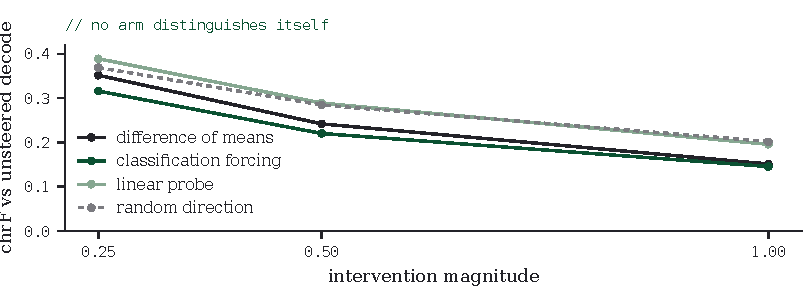
\includegraphics[width=\linewidth]{figures/fig-naturalness.pdf}
\caption{chrF between steered and unsteered decodes by intervention
magnitude. All four arms, the random direction included, damage the
decode at nearly the same rate; no arm buys naturalness at matched
magnitude.}
\label{fig:naturalness}
\end{figure}

The decisive comparison, though, is architectural. A single-layer grouped-softmax
SAE reproduces the Ontologizer's code structure, contrastive signature,
and text fidelity at better reconstruction with half the parameters. It
is the rival null hypothesis the full architecture must beat on
steering quality and task naturalness, and that comparison is where the
work currently sits.

\subsection{Seed stability}
\label{sec:prelim-seed}
Partitions do not reproduce across seeds at matched training. A second
run of the \texttt{resid\_nc\_hm} configuration from a different seed,
compared at matched training (370k steps on both sides), matches
essentially nothing
(Figure~\ref{fig:seed}): no head pair and at most $0.3\%$ of entries
clear a $0.3$ cosine threshold on dictionary geometry, and
activation-frame containment over a shared evaluation batch is at most
$0.001$ at any threshold, against $0.31$/$0.24$/$0.15$/$0.03$ for the
k32 SAE and its own seed replica across the four match thresholds
($0.3$--$0.9$). The metric itself has headroom: the same run compared
against itself $2{,}600$ steps apart scores $1.000$ on geometry at
every threshold, and $0.65$ at the loosest activation threshold
(falling to $0.20$ at the strictest), so the activation frame has a
self-ceiling well below one and the cross-seed numbers sit far below
both ceilings. At matched training the Ontologizer's partitions are
less reproducible across seeds than the SAE latents this proposal
criticizes. A replica carried to \texttt{resid\_nc\_hm}'s full $4.4$M
steps is the remaining control.

\begin{figure}[tp]\centering
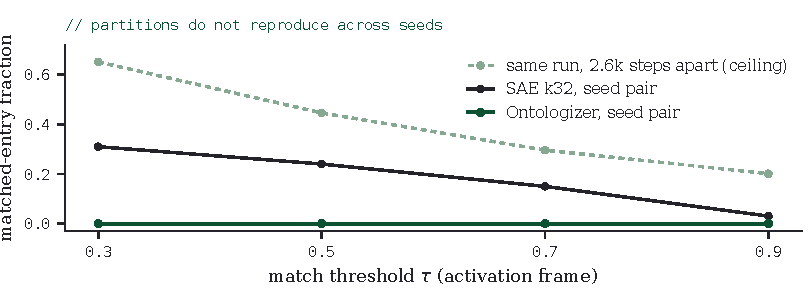
\includegraphics[width=\linewidth]{figures/fig-seed.pdf}
\caption{Cross-seed matched-entry fraction on the activation frame by
threshold. The same-run pair bounds what the metric can detect ($0.65$
at $\tau{=}0.3$); the k32 SAE pair reproduces partially; Ontologizer
partitions reproduce not at all.}
\label{fig:seed}
\end{figure}

\subsection{Development over training}
\label{sec:prelim-devinterp}
Tracking \texttt{resid\_nc\_hm}'s full 448-checkpoint history gives
the devinterp question a first answer. The tracked statistic applies
Table~\ref{tab:prelim-headcoh}'s $z$-score machinery to the refit
end-to-end direction matrix rather than to raw dictionary decode
directions, so the two are not directly comparable: the notes' raw
decode directions repel ($z{=}{-}17.6$, measured on \texttt{resid\_nc}
at 372.6k steps) while the refit directions on
\texttt{resid\_nc\_hm}'s final checkpoint cohere ($z{=}{+}72$); the
statistics differ in both instrument and substrate, and the refit
frame folds in the shared decoder and cross-layer interactions. On that statistic the
shape is rise, peak, and partial relaxation
(Figure~\ref{fig:devinterp}): mean within-head $z_{\cos}$ climbs from
$1.8$ at step 10k to a peak of $119$ near step 370k (median $123$,
every head above $z{=}2$), then relaxes over the remaining $4$M steps
to $72$ at the final checkpoint (median $105$, $0.79$ above $z{=}2$).
The code itself moves the other way after the annealing transient:
per-sample entropy returns to $4.5$ bits of a $5$-bit maximum and usage
KL falls toward uniform: relative to initialization the consolidation
is in the geometry the classifications write, while the classifications
themselves stay soft.

\begin{figure}[tp]\centering
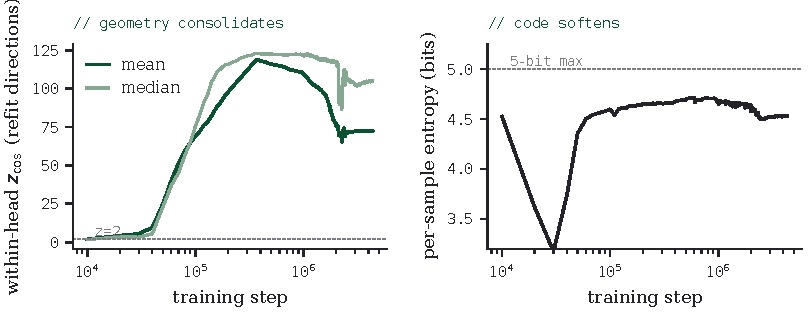
\includegraphics[width=\linewidth]{figures/fig-devinterp.pdf}
\caption{The 448-checkpoint training history. Left: within-head
coherence of refit end-to-end directions, $z$-scored against
size-matched nulls; rise, peak near step 370k, partial relaxation.
Right: mean per-sample classification entropy returns toward the
$5$-bit maximum after the annealing transient. Geometry consolidates
while the code itself stays soft.}
\label{fig:devinterp}
\end{figure}

\subsection{HSIC-bottleneck ablation}
\label{sec:prelim-hsic}
An HSIC bottleneck is a candidate replacement for the auxiliary
losses: maximize dependence with the reconstruction target while
penalizing dependence between heads. Both arms are in, retrained on
the \texttt{resid\_nc\_hm} configuration to 372k steps. Replacing the
four auxiliary terms with the HSIC objective destroys head health: a
late, persistent freeze takes 77 of 160 heads by the final checkpoint,
one layer entirely (layer 3, 32/32 from step 80k), while
reconstruction lands slightly behind the control (tail-mean training
MSE $3.7{\times}10^{-5}$ against $3.4{\times}10^{-5}$). Adding HSIC on
top of the auxiliary terms is worse on both counts: reconstruction
$4.4{\times}10^{-5}$, and 41 of 160 heads still frozen at the end,
layer 3 fully frozen by 80k with only partial thaw
(Figure~\ref{fig:hsic}). The failure mode is \texttt{resid\_nc}'s late
freeze, not the transient, which places the bottleneck and the
mean-entropy bonus in direct opposition: the bonus prevents exactly
what HSIC induces. As formulated the bottleneck is not a replacement,
and it is not an addition either.

\begin{figure}[tp]\centering
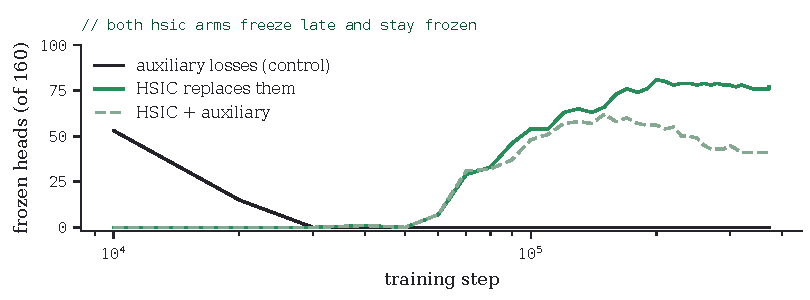
\includegraphics[width=\linewidth]{figures/fig-hsic.pdf}
\caption{Total frozen heads over training for the three loss
configurations, all on the \texttt{resid\_nc\_hm} configuration at
372k steps. The auxiliary-loss control's freeze is the early transient
and resolves; both HSIC arms develop the late, persistent freeze
instead, and the auxiliary terms only partially thaw it.}
\label{fig:hsic}
\end{figure}

\subsection{Against the desiderata}
Scored against the introduction: causal is currently positive (the
forced-classification steering result is causally verified), composable
is positive (interventions compose approximately additively), and
closed-form is negative (parameter-space decodes fail as descriptions).
Seed stability is measured on both sides: the k32 SAE pair matches at
$0.31$ down to $0.03$ as the threshold tightens while Ontologizer
partitions match at zero (Section~\ref{sec:prelim-seed}). The residual
stack's one quantified credit remains roughly $3\times$ adaptive
compensation under truncation (the shrinkage decomposition in the
working notes). Of the outstanding comparisons, the
steering overlay is a qualified positive, task naturalness is so far a
wash, and seed stability is a clear negative; the reconstruction price
Table~\ref{tab:prelim-pareto} puts on the architecture stands.



\section{Future work}

\subsection{Completing the evaluation}
\label{sec:future-completing}
The steering overlay, task naturalness, partition-level seed stability,
and the training-history diagnostics are reported above; cross-model
feature splitting and sparse language probing are covered in the notes
and not repeated here. What remains of the deciding set: human scoring
of the blinded naturalness sheet, the full-length seed replica, and the
fresh-encoded evaluation set. The last is blocked: the deterministic
mC4 stream is exhausted by the 4M-sample training cache, so no held-out
tail exists and closing the train/eval asymmetry requires a different
source (the C4 validation split is the leading candidate). The
controlled retrains and the HSIC arms are reported above
(Figures~\ref{fig:variants} and~\ref{fig:hsic}). Beyond the deciding
set, three comparisons remain open: the grouped-softmax rival on
steering quality, the RL decode-cycle tier and its convergence race,
and full-length scaling retrains.

\subsection{Change in interpretability over training}
First numbers are in Section~\ref{sec:prelim-devinterp}. The remaining
work is aligning the per-layer sharpening curves with independently
estimated stage boundaries, which needs the boundary estimator rather
than new tracking machinery.

\subsection{Transcoder adaptation}
The architecture currently reconstructs an embedding. Adapting it to map
between layers, as transcoders do, is the obvious next target.

\subsection{HSIC bottleneck}
The measured ablation is in Section~\ref{sec:prelim-hsic}. Whether a
reformulated bottleneck can coexist with the load balancing the
mean-entropy bonus provides is open.



\section*{Acknowledgements}
Design, typesetting, and editorial production of this preprint are by
The Flock Capital Research Department, whose error-diffusion pipeline
also printed the plates.

\printbibliography

%\input{sections/appendix.tex}

\vspace{20pt}
\noindent\plate{
\includegraphics[width=\textwidth]{figures/end-ridge.png}}\\[3pt]
\mutedlabel{ridge \textperiodcentered{} seed 32 \textperiodcentered{} the same pipeline, closing the file}

\end{document}
